\newpage
\section{Sable}

\begin{figure}[h]
    \centering
    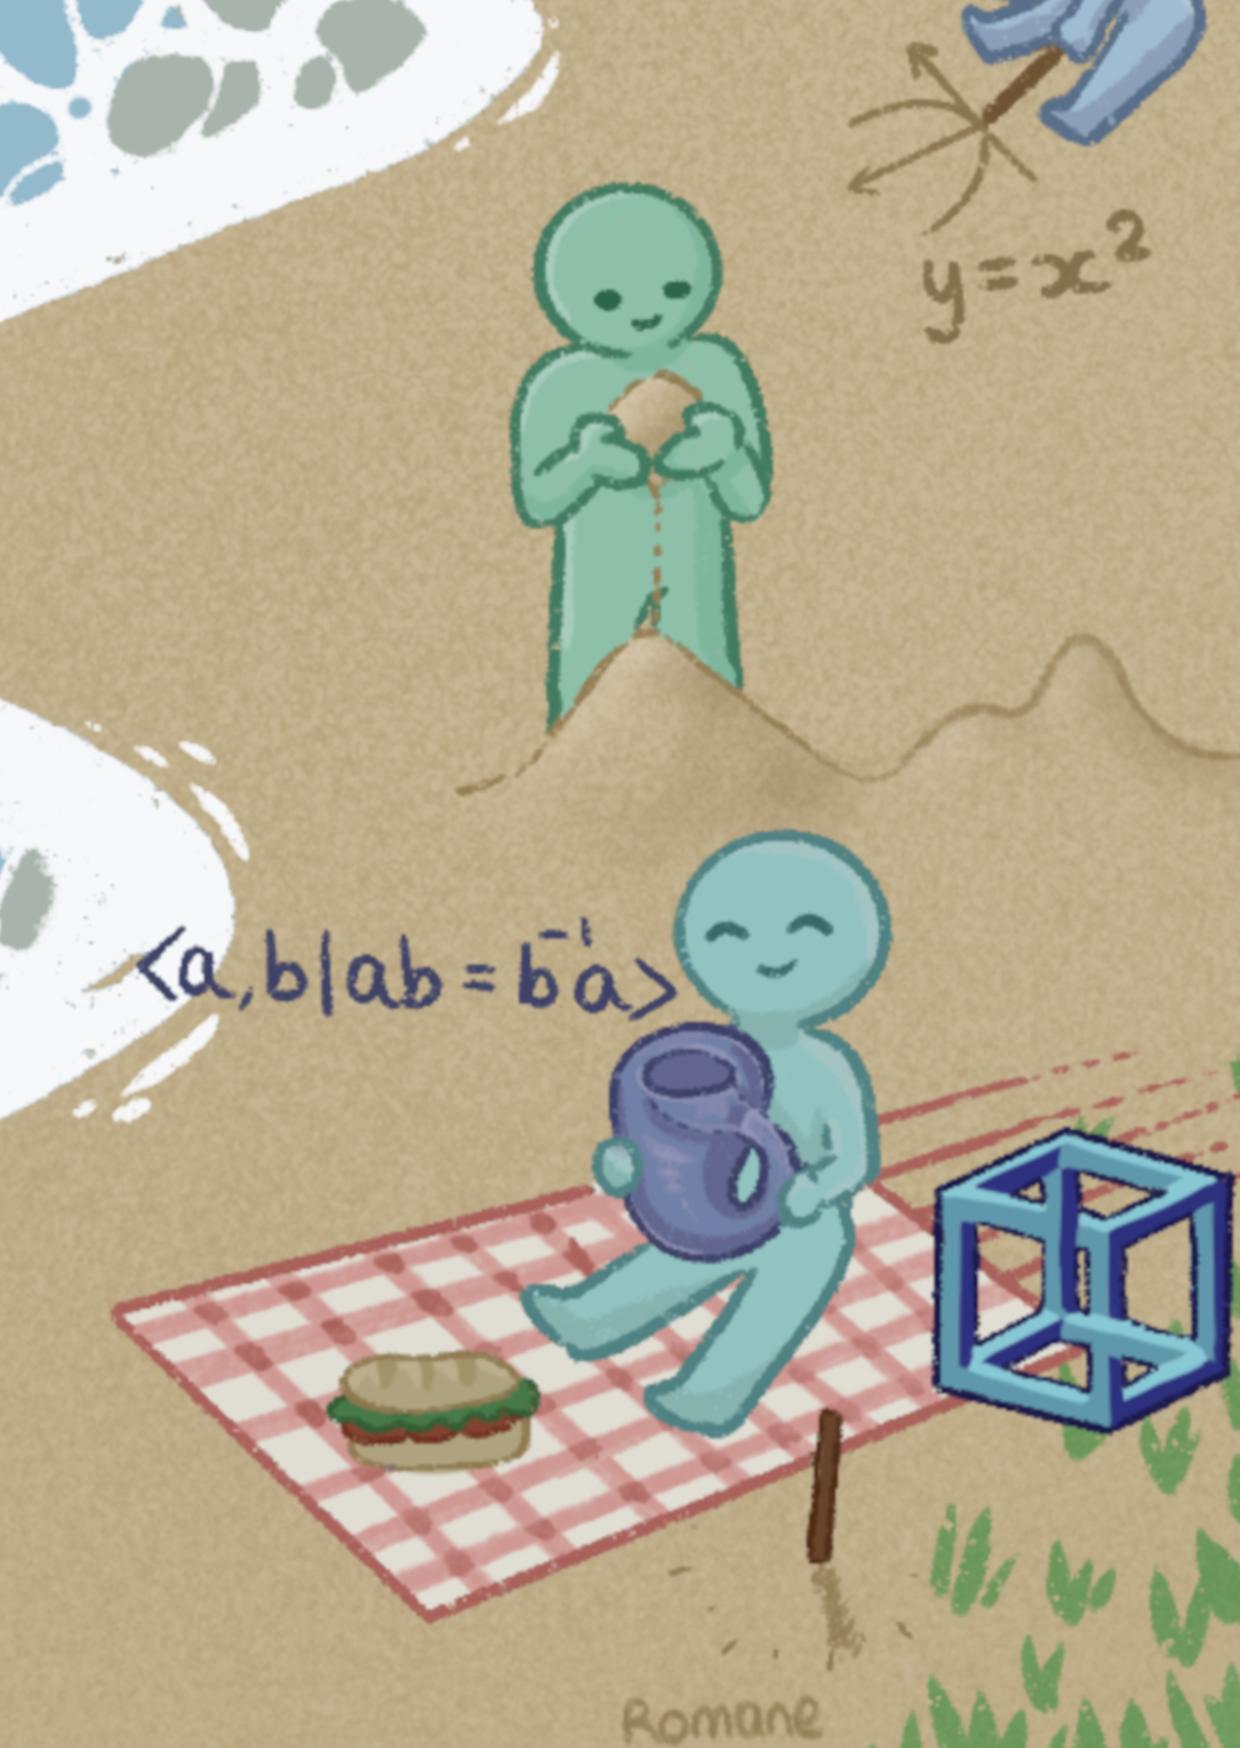
\includegraphics[height=0.5\textheight]{Cartes_postales/carte03-sable.png}\label{fig:c03}
    \caption{Carte postale: Sable}
\end{figure}

Les tas de sable ont des propriétés physique très intéressantes. Si on laisse tomber des grains de sable verticalement, on obtient un cône. Et l'angle au sommet de ce cône, appelé angle de repos, dépend à la fois de la gravité et des forces de frottements qui font que les grains de sable s'accrochent entre eux. En tombant, trois choses peuvent arriver: le tas de sable grossit, le grain déclenche un petit glissement, ou, très rarement, le grain déclenche une avalanche massive et une grande partie du tas s'effondre.

\medskip

On appelle ce genre de système un système critique: une petite variation locale peut entraîner des conséquences globales majeures. En mathématiques, on peut créer des modèles permettant de représenter ce genre de phénomène, et on peut estimer à quel point on est proche de ce seuil critique où une avalanche peut arriver. C'est très utile quand on part au ski!



